\documentclass[10pt]{article}

\usepackage[margin=1in]{geometry}
\usepackage{textcomp}
\usepackage{parskip}
\usepackage{amsmath}
\usepackage[backend=biber, style=alphabetic, sorting=ynt]{biblatex}
\usepackage{graphicx}
\usepackage{wrapfig}

\graphicspath{{./images/}}

\addbibresource{paper.bib}

\begin{document}

\section{Objective}

In experiments for dark matter detection, one of the most important and challenging hurdles to overcome is that of background radiation. Unwanted particles from a variety of sources can produce event signatures that appear very similar to those of dark matter candidates.

To resolve this, physicists must determine a discriminator function that can, based on some sensory data, separate dark matter candidates from background radiation. Two general problems stand in the way:

\begin{enumerate}
    \item A detailed model of the physical environment is often used to produce an accurate discriminator. This takes a long time even for a team of experienced physicists, and will have to be updated whenever the physical variables of the experimental apparatus change.

    \item The primary intention of many dark matter experiments, which is to reduce background radiation to the lowest level possible, means that there will be a very small number of background events detected. This places a severe limit on the amount of data that is available to optimize such a discriminator.

    Furthermore, what little data is available to optimize a discriminator very often contains impurities, because whatever background radiation is present during WIMP detection runs is also present during calibration runs. These are difficult to separate without already having access to a functional discriminator, creating a ``chicken or the egg'' problem (from which a common way to escape is to create a time- and labor-intensive simulation).
\end{enumerate}

The objective of this study is to explore a potential methodology that resolves both of these problems using techniques based on machine learning. These include supervised learning algorithms that learn to separate calibration data sets, and semi-supervised learning algorithms that simultaneously learn an effective discriminator and improve the purity of their own training data sets.

\section{Previous PICO-60 Analysis}

\subsection{Background}

The PICO-60 bubble chamber experiment for detection of weakly interacting massive particles (WIMPs) was completed in 2017. It provides an excellent basis on which to develop and test the efficacy of such techniques as a potential tool for event discrimination, relative to the conventional techniques used during initial analysis of the experiment.

WIMP candidates in the cross section and mass ranges that the PICO-60 detector is sensitive to are predicted to produce nuclear recoils with the same properties as those created by neutrons. The key difference is that neutrons frequently (but not always) scatter and produce multiple bubbles, where the extremely small predicted cross sections of WIMP candidates mean that they should almost invariably create just one bubble. This means single-bubble neutron events can be used to optimize a discriminator to detect WIMP events.

The approximate expected ratio between single-bubble and multiple-bubble events generated by neutrons is known. A measured quantity of single-bubble events generated by nuclear recoils, in excess of this prediction, would be indicative of WIMP interactions. Consequently, it is imperative to isolate only those events associated with nuclear recoils.

\subsection{Discrimination Techniques}

\subsubsection{Overview}

In this study, newly developed methodologies were compared to the 2 discrimination techniques developed previously for the PICO-60 experiment: Acoustic Parameter and machine learning.

\subsubsection{Acoustic Parameter}

Acoustic Parameter is the technique used for event discrimination in the original PICO-60 analysis. It is a function that discriminates between alpha particles and nuclear recoils based on audio data. It was derived based on a physical model of the bubble chamber, and was tuned using calibration runs using neutron sources to produce events in the PICO-60 apparatus.

Before Acoustic Parameter can be calculated, the audio data must first be converted into the frequency domain (specifically, with the banded Fourier transform $\beta_{8}$). It must also be preprocessed with the position correction function $PosCor(\beta_{8}, \chi)$, which adjusts the overall volume of an audio recording according to its position in the vessel. This is done because the resonance characteristics differ significantly depending on the position of an event.

Finally, a set of data cuts must be applied to remove certain classes of events which are not accurately classified by Acoustic Parameter. These classes include wall event and multiple-bubble events.

These conversion, preprocessing, and data cutting steps were reapplied during this study, and are described in section \ref{data_formats}.

\subsubsection{Machine Learning}

As part of the PICO-60 experiment, some testing was conducted to determine whether machine learning (in the form of a multi-layer perceptron) could be a viable technique to consider for a discrimination function. The results, while not definitive, indicated that the general technique warranted further investigation.

\subsection{Data Sources and Formats} \label{data_formats}

Discriminators can use a variety of different data formats to make predictions. These are collected from the two essential sensors present in the PICO-60 apparatus: piezoelectric microphones (piezos) and cameras.

\subsubsection{Piezo-Derived}

\textit{Raw Waveform}

The lowest-level data derived from the piezos is the raw waveform $\omega$. $\omega$ consists of a series of samples collected every 400,000\textsuperscript{th} of a second. They are each represented as a 16-bit integer. Only the section of the audio between sample 90,000 (inclusive) and sample 190,000 (exclusive) was used during most experiments, because before this there is background noise, and afterwards there is a clipped signal produced by hydraulics repressurizing the vessel. (These sections contain no information and can be undesirably fit on by neural networks.)

\textit{Fourier Transform}

The raw waveform $\omega$ was converted into the frequency domain by means of a 1-dimensional Discrete Fourier Transform for real input. Since DFTs produce sequences of complex numbers, the magnitude of each element was computed. The full-resolution Fourier transform $\beta _{50,001}$ consists of a sequence of complex numbers, half the length of the raw waveform $\omega$.

Beyond this, the banded Fourier transform $\beta_{8}$ (which is the input to Acoustic Parameter and the original neural analysis) was computed by integrating the resonant energy over all frequencies within each of a set of bands. This can be thought of as a method of signal downscaling, compressing the signal into a smaller number of data points.

\begin{figure}[h]
    \centering
    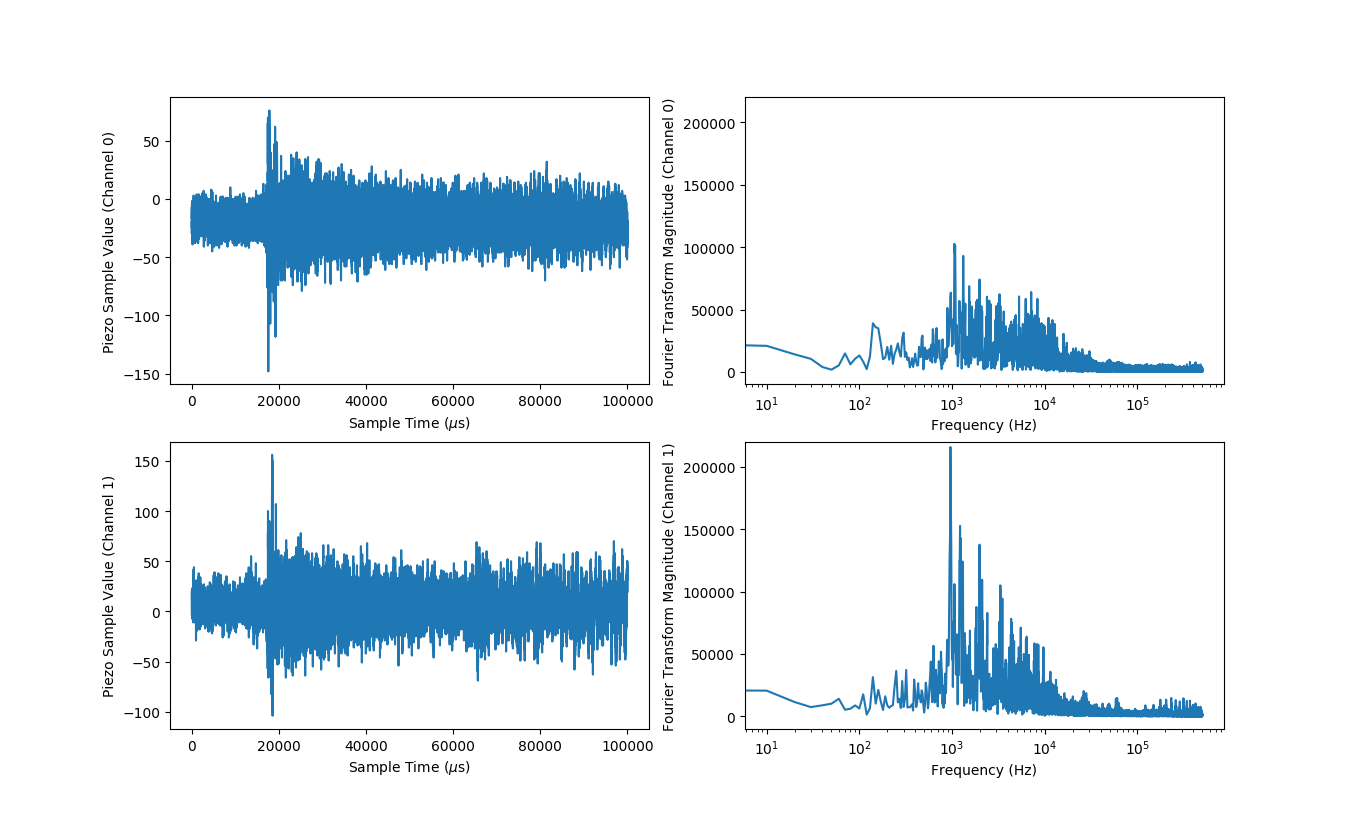
\includegraphics[width=\textwidth]{audio}
    \caption{\label{} An example of the cropped audio waveform $\omega$ and full resolution Fourier transform $\beta_{50,001}$.}
\end{figure}

\subsubsection{Camera-Derived}

\textit{Image Window Sequence}

For each event that is captured, the 4 cameras within the PICO-60 apparatus each capture a sequence of 71 images before and after formation of a bubble is detected. These raw images contain a large amount of extraneous information; they encompass the entire vessel. To reduce the input information, the image window sequence $\iota$ includes 50\texttimes50 cropped windows around the position of the bubble. The 71 frames, many of which contain either no bubble or a bubble in later stages of formation, are reduced to 10 immediately around the formation of the bubble. $\iota$ includes 5 frames from before the recording trigger, because the bubble does not cause a trigger until it is already at a significant size.

\begin{figure}[h]
    \centering
    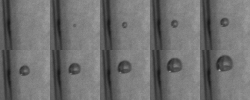
\includegraphics[width=0.7\textwidth]{image_grid}
    \caption{\label{} An example of the image sequence $\iota$.}
\end{figure}

\textit{3D Position}

The 3-dimensional position $\chi$ of the bubble within the vessel is calculated using triangulation, based on the known positions and angles of the cameras and the position of the bubble within the field of view of each camera. This is used in the banded frequency position correction function $PosCor(\beta _{8}, \chi)$, which corrects $\beta _{8}$ for variations in amplitude which depend on the position of the bubble.

\subsection{Data Cuts}

Techniques in this study are trained and validated on a number of different data sets. The selection of these sets focused on the fundamental trade-off between quality and quantity of data; by setting a higher standard for the validity of training data, one has less data to train on.

The initial data set $D$ to which these cuts are applied consists of all events recorded during PICO-60 run 2.

\subsubsection{Basic Quality Cut}

A certain number of cuts are necessarily applied to all data to ensure meaningful results. Otherwise, significant overfitting on biases in the data is likely. This basic quality cut $QualCut(D)$ consists of the following restrictions:

\begin{itemize}
    \item The run was not collected during engineering or testing ($\texttt{run\_type}\neq99$)
    \item Recording was triggered by the camera ($\texttt{trigger\_main}=0$)
    \item Acoustic Parameter is not erroneously large and negative ($log_{10}(\texttt{acoustic\_bubnum})>-100$)
    \item Recorded more than 25 seconds after reaching target pressure ($\texttt{te}>25$)
    \item The bubble position $\chi$ was successfully calculated ($[\chi_{X}, \chi_{Y}, \chi_{Z}]\neq[-100, -100, -100]$)
\end{itemize}

\subsubsection{Bubble Multiplicity Cut}

PICO-60 events which include multiple bubbles are \textit{always} neutron events; alpha particles and WIMP candidates never scatter. Thus, no discriminator is required to handle these events, so they are removed. The bubble multiplicity cut $MultiCut(D)$ consists of the following restrictions:

\begin{itemize}
    \item Either 0 or 1 bubbles are detected based on images from the camera ($\texttt{nbub}<2$)
    \item The number of bubbles approximated using the pressure transducer is close to 1 ($0.7<\texttt{dytranCZ}<1.3$)
\end{itemize}

\subsubsection{Wall Cut}

Events that occur near the walls of the vessel have acoustic properties which are notably different from events nearer the center of the vessel. It can be desirable for a discriminator to handle these events correctly; however, Acoustic Parameter does not, and neither does the neural network used in the previous PICO-60 paper. Thus, removing wall events allowed for a more meaningful direct comparison between a new neural network and existing techniques.

The complete wall cut $WallCut(D)$ is a composition of the fiducial cut $FidWallCut(D)$ (which makes use of the 3D position $\chi$), the pressure cut $PresWallCut(D)$ (which uses data from the pressure transducer), and the acoustic cut $AcWallCut(D)$ (which uses the banded Fourier transform $\beta _{8}$).

\textit{Fiducial Cut}

The fiducial cut $FidWallCut(D)$ defines an spatial area along the walls of the vessel within which no events are accepted. It makes use of the bubble position $\chi$, the distance from the bubble to the center of the vessel $R$, and the distance from the bubble to the nearest wall, which is defined as $min(\texttt{Dwall}, \texttt{Dwall\_horiz})$. It is defined as follows:

\begin{itemize}
    \item $Z \leq 523$
    \item Any of the following 4 restrictions are true:
    \begin{itemize}
        \item $(min(\texttt{Dwall}, \texttt{Dwall\_horiz}) > 6) \land (0 < \chi_{Z} \leq 400)$
        \item $(min(\texttt{Dwall}, \texttt{Dwall\_horiz}) > 6) \land (\chi_{Z} \leq 0) \land (R \leq 100)$
        \item $(min(\texttt{Dwall}, \texttt{Dwall\_horiz}) > 13) \land (\chi_{Z} \leq 0) \land (R > 100)$
        \item $(min(\texttt{Dwall}, \texttt{Dwall\_horiz}) > 13) \land (\chi_{Z} > 400)$
    \end{itemize}
\end{itemize}

\textit{Pressure Cut}

The pressure cut $PresWallCut(D)$ restricts the pressure detected by the pressure transducer, without any position corrections, to be close to 1 ($0.7<\texttt{dytranC}<1.3$). In combination with the acoustic cut $AcWallCut(D)$, this acts as a backup to the fiducial cut.

\textit{Acoustic Cut}

The acoustic cut $AcWallCut(D)$ is defined using the banded Fourier transform $\beta_{8}$ as follows:

$45 < mean(\beta_{8}[(0, 2), (0, 1)]) < 300$

This takes advantage of differences in the frequency distribution (specifically the first and second frequency bands of the first and third piezos) of wall events and non-wall events.

\begin{figure}[h!]
    \centering
    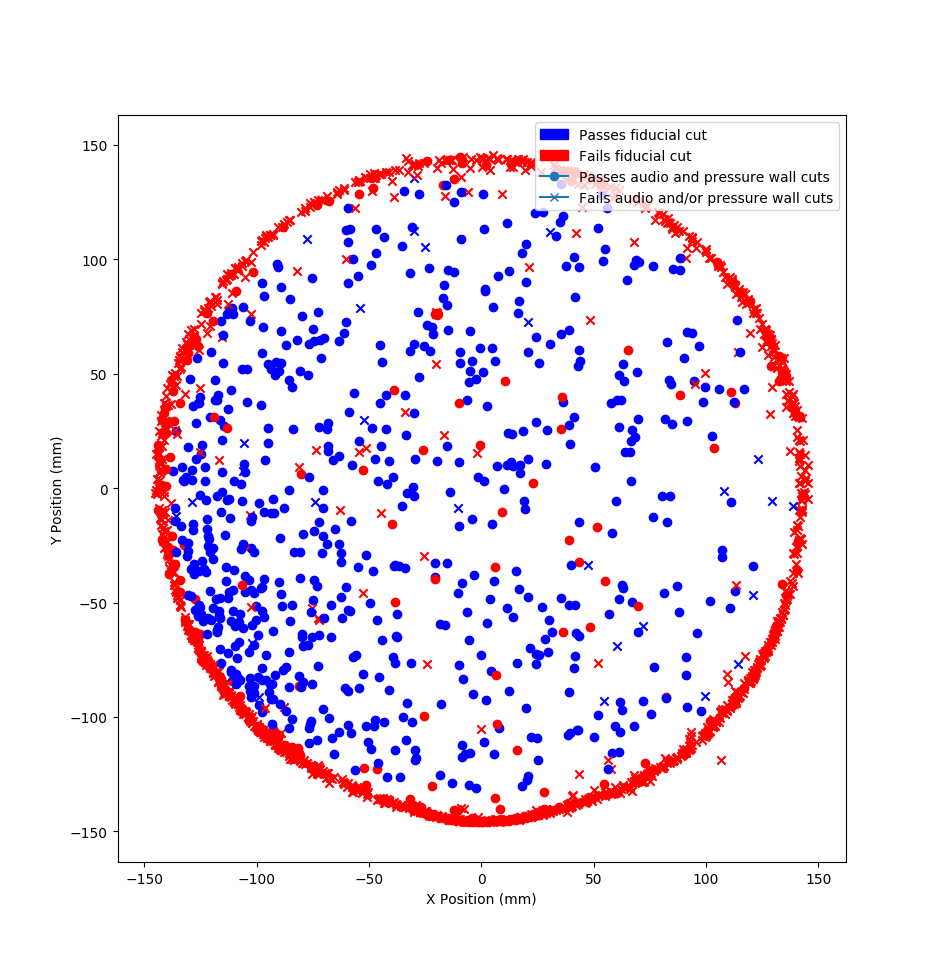
\includegraphics[width=\textwidth]{wall_event_positions}
    \caption{\label{} A visualization of the fiducial cuts and how they match up with the pressure and acoustic cuts.}
\end{figure}

\section{Machine Learning Techniques}

\subsection{Background}

While machine learning has existed for many years, recent developments in artificial neural networks have opened up a wide variety of applications and fields in which it can now be used.

One of the key benefits of machine learning systems is that they have the capacity to approximate arbitrary functions (such as Acoustic Parameter) without human intervention. This greatly alleviates the need for human programmers to define and optimize the exact algorithm used.

This characteristic has already shown wide-ranging implications in many fields. For one, it has the potential to drastically increase the speed of iteration for the people working on a project, since retraining a machine learning system when a hardware or software variable changes is much faster than calibrating a human-designed model.

\subsection{Techniques Considered}

Machine learning techniques are usually divided into two main categories:

\begin{itemize}
    \item Supervised learning, in which a system is trained on a set of labeled data to classify unseen examples according to the patterns it observes in the training set. The training set is very important; biases and errors often slow training and produce worse results.
    \item Unsupervised learning, in which a system finds patterns or clusters in a set of unlabeled data. This can find order in almost any training set, but it is unpredictable and may not find the particular patterns it is expected to find.
\end{itemize}

A significant challenge in this application is that neither supervised nor unsupervised learning is ideal. The calibration sets available for training are not pure, so supervised learning is likely to overfit on biases and produce undesirable results. Conversely, unsupervised learning may be able to find clusters in the data, but it is impossible to guarantee it will distinguish between nuclear recoils and alpha particles as opposed to some other binary separation.

For these reasons, a technique is needed that is not as sensitive to problematic training data as supervised learning, but more predictable and controllable than unsupervised learning. Semi-supervised learning is a middle ground in this regard. It makes use of a labeled set as well as an unlabeled set. It uses the labeled set for training, and uses the unlabeled set to further structure the patterns it finds in the training set (which may not be sufficiently large to apply to supervised learning).

2 semi-supervised algorithms were developed and implemented for this study: gravitational differentiation and iterative cluster nucleation. Both are discussed in detail in section \ref{semi_supervised}.

\subsection{Optimization Process}

Learning algorithms in this study are optimized systematically, with a variety of neural network configurations and input formats. To obtain meaningful results, it is important to minimize the number of variables during each individual run. Thus, since the 2 semi-supervised algorithms incorporate neural network models, it is important that the input formats and other hyperparameters of these networks are optimized first to some degree. This means the task is split into 2 distinct phases:

\begin{enumerate}
    \item Develop and verify several different supervised learning systems. Their performance is evaluated based on their ability to replicate the ground truths they are trained on. While this does not produce an optimal discriminator, it does reveal architectures that are capable, in essence, of learning to accomplish the discrimination task.
    \item Using general supervised learning systems and input formats that were determined to be effective, optimize the hyperparameters of the semi-supervised learning algorithm to reproduce Acoustic Parameter as closely as possible. Since Acoustic Parameter is not used to optimize the neural network directly at any point, models that excel at this task demonstrate an ability to learn the desired discriminator while ignoring the impurities in the training set.
\end{enumerate}

\section{Supervised Learning}

\subsection{Overview}

Important unknowns to be determined through experimentation with supervised learning included the most effective input format for the network, and the associated general network structure. Three major such configurations were applied:

\begin{enumerate}
    \item A convolutional neural network trained on the raw waveform $\omega$.
    \item A dense neural network trained on banded Fourier transforms $\beta_{N}$.
    \item A convolutional neural network trained on the image window data $\iota$.
\end{enumerate}

Except where specifically mentioned, $WallCut(D)$ was not applied. This was done to test the network's ability to handle complex acoustic characteristics including resonance. There is a relatively clear-cut discrimination boundary in PICO-60, but this may not be the case in other applications.

\subsection{Performance Analysis}

The performance of supervised learning neural networks was evaluated using 2 metrics. One is a simple classification accuracy value, which corresponds to the number of validation examples the network classifies incorrectly. This effectively summarizes how often the network is outright correct or incorrect, but fails to capture how decisive it is.

A metric that captures this property is the class-wise standard deviation. This is a variable defined as $C$ below, where $N$ and $A$ are the sets of outputs of the supervised learning discriminator in question, corresponding to the sets of neutrons and alpha particles respectively. It calculates the spread of the network's predictions for each ground truth class. This means that a decisive discriminator, which produces a wide separation between the two classes, is preferred over one that produces a nebulous cloud of outputs with a seemingly arbitrary decision boundary.

$S=std(N \cup A)$

$C=(std(N \div S) + std(A \div S)) \div 2$

The first step is to calculate the standard deviation S of the union of the two sets. This gives an indication of the scale of the overall distribution. When $N$ and $A$ are divided by $S$, they are normalized so that the standard deviation of their union is equal to 1. While the neural network’s outputs are bounded in the range of 0 to 1 with a sigmoid activation, Acoustic Parameter has a significantly wider range. Normalization of the union prevents this from creating a bias where Acoustic Parameter would produce a higher standard deviation with a similarly proportioned error.

The second step is to calculate the mean of the standard deviations of the normalized sets of neutrons and alpha particles individually. This is an indication of how tightly clustered or widely dispersed the discriminator’s predictions are. Very consistent predictions of $x$ for neutrons and $y$ for alphas (for any $x$ and $y$), with minimal variance off of those specific values, will produce a low class-wise standard deviation.

\subsection{Convolutional Neural Network for Raw Waveform Analysis}

\subsubsection{Structure}

A convolutional neural network was used for analyzing the raw waveform $\omega$ directly, without any preprocessing whatsoever. This avoids any destruction of information, and should be possible, in theory, for a neural network to handle. For this task, a very deep (20 layers in its shallowest configuration) 1-dimensional fully convolutional neural network was applied. The architecture was inspired by the M34-res network \cite{verydeepconvnets} for analysis of raw waveforms. L2 regularization was used to alleviate overfitting, and batch normalization was applied to the input. (Its hyperparameters were modified significantly through manual empirical testing as well as grid searches.)

Two different configurations were tested:
\begin{enumerate}
    \item A configuration that operates strictly on $\omega$ with no position corrections of any kind (furthermore $DeepConv(\omega)$).
    \item A configuration with an additional position input on a lower layer such that it should be able to learn to incorporate position corrections into its outputs ($DeepConvWithPos(\omega, \chi)$).
\end{enumerate}

\subsubsection{Results}

During early tests with variations on $DeepConv(\omega)$, it was revealed to have an incredible capacity to separate run types based on unwanted biases. It was able to separate the AmBe calibration run from combined background runs with 96\% accuracy, and to separate all calibration runs from background runs with 91\% accuracy. This was determined to be caused by the network detecting and fitting on biases in the white noise at the beginning and hydraulic recompression sounds at the end of the raw waveform. This extraneous information was subsequently cropped out.

Once the audio was cropped properly, $DeepConv(\omega)$ achieved a maximum of 77\% accuracy on validation data. Using the same network architecture (except for the input layer), $DeepConvWithPos(\omega, \chi)$ achieved 85\%. The maximum obtained on a grid search with position input was 91\% (although with a high class-wise standard deviation of 0.61). While this is not a drastic improvement, it is a fairly strong indication that the network is able to extract meaningful information from the position, which may be used in an internal position correction of the volume.

However, the lack of decisiveness observed even when accuracy was relatively high, as seen in Figure \ref{waveform_best_validation}, implies this is a suboptimal technique.

\begin{figure}[h]
    \centering
    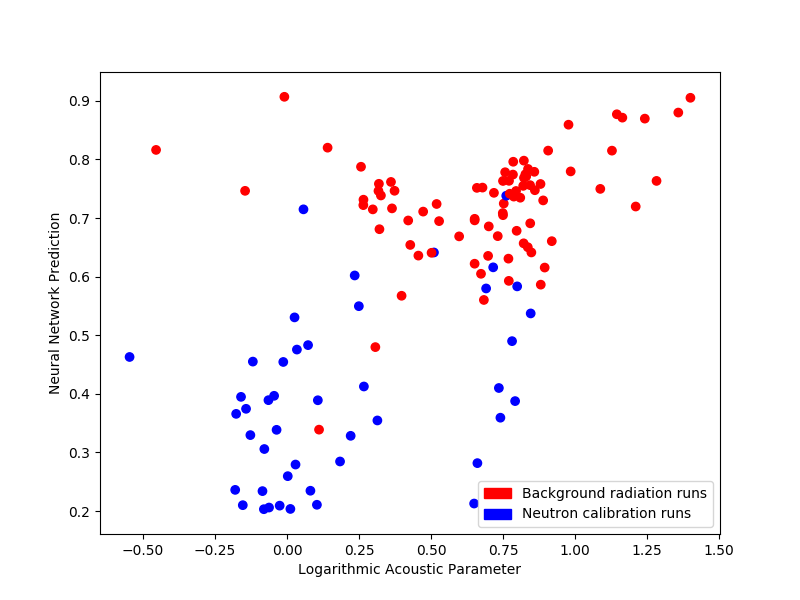
\includegraphics[width=\textwidth]{waveform_best_validation}
    \caption{\label{waveform_best_validation} Accuracy of $DeepConvWithPos(\omega, \chi)$ compared to Acoustic Parameter at discriminating between run types without $WallCut(D)$ (91\% accuracy).}
\end{figure}

\subsection{Multi-Layer Perceptron for Fourier Transform Analysis}

\subsubsection{Structure}

Preprocessing the audio by applying a Fourier transform may be advantageous. If the frequency distribution and overall volume are indeed the most important factors for discrimination, the network can gather them straight from the Fourier transform $\beta_{N}$ rather than having to analyze $\omega$ to extract this information.

In addition to the Fourier transform used in the original PICO-60 analysis, higher resolutions were computed by similar means. These included $\beta _{5}$, $\beta _{10}$, $\beta _{20}$, and $\beta _{40}$. Also, the full-resolution $\beta _{50,001}$ was input into a neural network directly, without any downscaling.

$WallCut(D)$ was applied to the low-resolution Fourier transforms during early experiments (since they were used for Acoustic Parameter) to minimize the number of variables between the neural network and a proven discriminator.

Once again, configurations with and without position input were tested. This time, position corrections were optionally included when position input was not used. The resulting configurations are furthermore referred to as $FourierMLP(\beta_{N})$, $FourierMLP(PosCor(\beta_{N}))$ and $FourierMLPWithPos(\beta_{N}, \chi)$. Several different resolutions $N$ of $\beta_{N}$ were used. While there were variety of network architectures tested, most had a small number of layers (on the order of 3), applied dropout and L2 regularization, and used batch normalization once again.

\subsubsection{Results}

It became evident very quickly that, without $WallCut(D)$, a high resolution was not required to get a high accuracy relative to the ground truth data. $FourierMLP(\beta_{8})$ managed an excellent 98\% validation accuracy, and also produced a mean class-wise standard deviation of 0.29. Increasing the number of bands, even up to $FourierMLPWithPos(beta_{20}, \chi)$, did not improve the results; accuracy only reached 95\%, with an increased mean standard deviation of 0.42.

\begin{figure}[h]
    \centering
    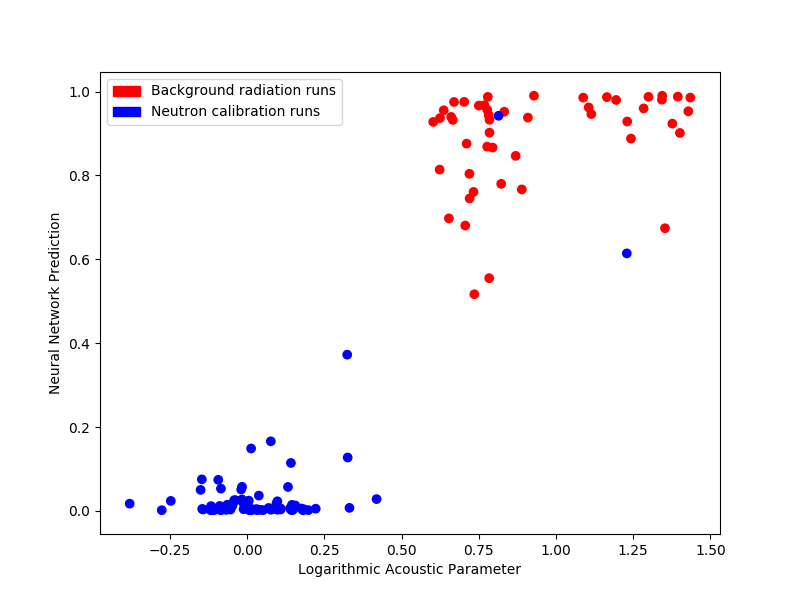
\includegraphics[width=\textwidth]{fourier_mlp_no_correction}
    \caption{\label{fourier_mlp_no_correction} Accuracy of $FourierMLP(\beta_{8})$ compared to Acoustic Parameter at discriminating between run types (98\% accuracy).}
\end{figure}

Unlike for the convolutional neural network trained on $\omega$, position input did not improve performance at all. In fact, $FourierMLP(\beta_{8})$, performed better than $FourierMLPWithPos(\beta_{8}, \chi)$, which reached only 95\% validation accuracy. Nevertheless, they both performed better than any of the network architectures trained on $\omega$.

The higher resolution demonstrated significant power when $WallCut(D)$ was not applied, and only \\ $QualCut(MultiCut(D))$ was used. $FourierMLPWithPos(\beta_{20}, \chi)$ achieved only 92\% accuracy (2 percentage points lower than the same configuration without $WallCut(D)$). $FourierMLPWithPos(\beta_{40}, \chi)$ also managed 92\% validation accuracy. However, training on $\beta_{50,001}$, which does not incorporate any banding, improved this figure to a maximum of 97\%. However, that epoch had a relatively high standard deviation, at 0.47.

\subsection{Convolutional Neural Network for Image Window Analysis}

\subsubsection{Structure}

It is an open question whether or not there is any information in the image data $\iota$ that could be used to distinguish between particle classes. Relative to the extremely short period of time in which the bubble forms (on the scale of nanoseconds), the framerate of the camera (340Hz) is extremely slow. While the very early stages of bubble formation (when the sound is produced) are known to differ depending on whether the bubble was created by a nuclear recoil or an alpha particle, it is unknown whether any visually apparent differences persist when the bubble is visible.

In an effort to resolve this, a 2-dimensional convolutional neural network was applied to the task of discriminating based on $\iota$. The network architecture consists of a moderate number of convolutional layers (on the scale of 9) and 3 dense layers at the end. L2 regularization was used on all layers, and dropout was additionally used on the dense layers. No position input is used (since there are no microphones that would require position correction), so the basic configuration is $ImageConv(\iota)$.

\subsubsection{Results}

Throughout a variety of different network architectures, the best validation accuracy obtained was 85\%. The corresponding training accuracy of 100\% indicates that severe overfitting is taking place. Also, the class-wise standard deviation was a very high 0.95, which implies its decisions are nearly random (as is apparent in \ref{image_window}). It is likely fitting on some form of noise within $\iota$. The fact that throughout many trials (including a grid search), no good performance on validation data was observed, provides significant evidence that images provide insufficient information for effective discrimination.

\begin{figure}[h]
    \centering
    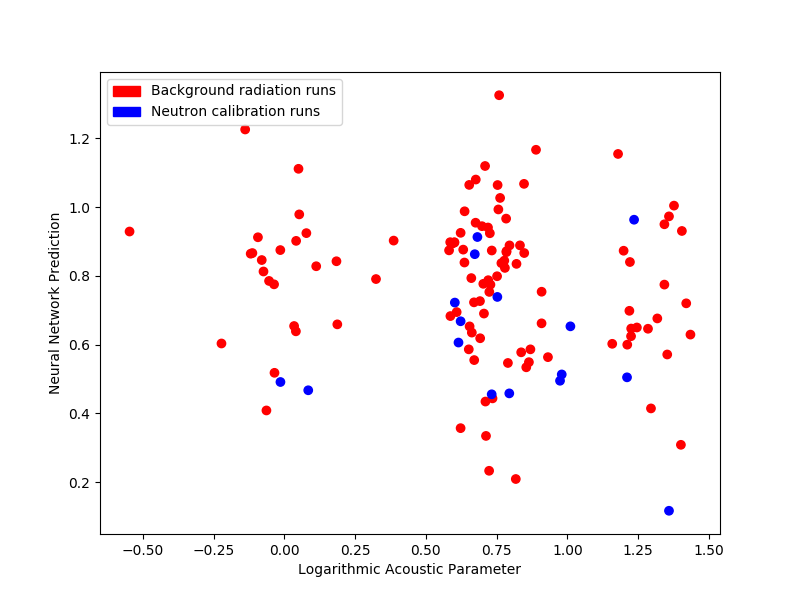
\includegraphics[width=\textwidth]{image_window}
    \caption{\label{image_window} Accuracy of $ImageConv(\iota)$ compared to Acoustic Parameter at discriminating between run types (85\% accuracy).}
\end{figure}

\subsection{Performance Summary}

The following table compares the accuracy and mean class-wise standard deviation values of various supervised learning configurations, with the original PICO-60 neural network provided as a baseline:

\begin{tabular}{|l|l|l|}
    \hline
    Configuration & Max Accuracy & Mean Class-Wise Standard Deviation \\
    \hline
    $DeepConv(\omega)$ & 77\% & TODO \\
    \hline
    $DeepConvWithPos(\omega, \chi)$ & 91\% & TODO \\
    \hline
\end{tabular}

\section{Semi-Supervised Learning} \label{semi_supervised}

\subsection{Overview}

Semi-supervised learning is the idea of training a machine learning model on a set of labeled data in addition to a set of unlabeled data. This has the advantage of requiring fewer labels to be collected than conventional supervised learning. However, it also has a very powerful advantage when training data is impure and the function to be learned is relatively simple (not simple in that it can be easily calculated by a person, but simple in that it does not require a huge set of training data). It allows a neural network to reinforce its own decisions.

In both of the semi-supervised learning algorithms applied, to arrive at an effective discriminator, the network first trains on a smaller amount of imperfect data. Because the ground truth data is imperfect, training on a relatively small set for a short period of time (potentially using regularization, in addition) ensures that the network will be less likely to overfit and its learned function will be simpler. This is in line with the objective, since, assuming the training inputs are normalized correctly, it should be simpler to discriminate between classes of particles than calibration runs.

The essence of these 2 algorithms, then, is a positive feedback loop in which, by using the network's most confident predictions in the training process, the desired (simpler) function is reinforced, when a conventional supervised learning system would have learned the more complex function that is taught by the ground truths.

In addition to improving performance with a labeled set known to be adequate, a goal of this category of techniques is to minimize the amount of labeled data necessary. This means less time must be spent on collection of calibration data, which can be a very slow process. Regularization techniques, which permit effective training on smaller sets, are applied with this purpose.

\subsection{Performance Analysis}

One of the main purposes of semi-supervised learning is to handle the impure training data effectively, and learn to replicate the imperfectly represented underlying pattern (nuclear recoils versus alpha particles) rather than merely fitting to separate run types. Therefore, performance is quantified by how accurately a system is able to replicate Acoustic Parameter, rather than simply reproduce the labels provided.

\subsection{Gravitational Differentiation}

\subsubsection{Concept}

Gravitational differentiation is a novel technique for gradient computation in the final layer of a neural network. It is intended for training a neural network in a semi-supervised fashion on a relatively small set of imperfectly labeled data, while simultaneously incorporating the network's changing predictions on a set of unlabeled data to encourage decisive classifications.

\subsubsection{Structure}

It makes use of the gravitational differentiation function $GravDiff(p, \psi, g)$, which is parameterized by the network's existing prediction $p$ on the training example in question, the degree $\psi$ of the piecewise exponential function used to distort the response of the gradient, and the gravitational multiplier $g$. The function is defined as follows:

$GravDiff(p, \psi, g) = g \cdot sgn(p) \cdot abs(tanh(2(p - 0.5))) ^ \psi$

The essential purpose of $GravDiff(p, \psi, g)$ is to allow confidently classified unlabeled examples to influence the training process, pushing them further towards the classification they are already near (like gravity), while ensuring examples with low-confidence classifications do not have a significant adverse effect.

It can be considered a distortion of the hyperbolic tangent that flattens the central range and exaggerates the asymptote on either side. The network's prediction $p$ is first transformed so its range is 1 to -1 rather than 0 to 1 ($2(p - 0.5)$). Next, the sigmoidal hyperbolic tangent is applied, producing a value of 0 in the center and asymptotic slopes to -1 and 1 at the edges.

However, what is really desired is a shallow slope in the center (so low-confidence network outputs in the range of, for instance, 0.2 to 0.8 will produce very shallow output gradients). Applying a relatively large exponent (on the order of 9) accomplishes this, because values less than 1 will rapidly approach 0. However, this only works with odd integer exponents (because they produce negative outputs for negative inputs), limiting the ability to fine-tune this function by changing $\psi$. To resolve this, a piecewise exponential function is used, where the absolute value is taken prior to applying the power and the sign is multiplied in afterwards. This permits use of the full range of curves produced by even and non-integer values of $\psi$.

This function is applied in a training algorithm that is parameterized by the set of imperfectly labeled data $\varsigma$, the set of unlabeled training data $\upsilon$, a binary classification neural network $NN(x)$ (where $x$ is the input data format), and the gravitational multiplier increment $\delta_g$. The distortion power $\psi$ is assumed to be constant throughout a training run, and the gravitational multiplier $g$ is initialized at 0, gradually increasing during training. It iterates as follows:

\begin{enumerate}
    \item Train $NN(x)$ for a single epoch on the combined set $\varsigma \cup \upsilon$, using the predefined ground truths for $\varsigma$ (with a mean squared error loss function) and the most recently calculated gravitational gradients for $\upsilon$.
    \item Calculate predictions $p$ with $NN(x)$ on the entirety of $\upsilon$. Calculate $GravDiff(p, \psi, g)$ and record the resulting gradients for the next iteration.
    \item Increment $g$ by $\delta_{g}$. At the beginning, when $g = 0$, training will be entirely based on the labeled set $\varsigma$, and progressively, over the course of a run, the gravitational effect increases with $g$.
\end{enumerate}

This system was trained using $FourierMLP(\beta_{8})$ for $NN(x)$, because this was the most successful configuration in supervised learning. It produced the highest accuracy as well as the lowest class-wise standard deviation.

\subsubsection{Results}

During a grid search of parameters of the gravitational differentiation algorithm (in addition to the stochastic gradient descent learning rate), the algorithm achieved a maximum of 98\% validation accuracy. The mean over that run (also the highest overall) was 96\%.

Figure \ref{grav_opt_validation} shows the highly accurate replication of Acoustic Parameter. However, the examples that are classified incorrectly seem to have no correlation with Acoustic Parameter, suggesting that the learned function cues on different properties of the audio. While the discriminator may still be accurate, this property implies it may be less predictable when trained on new data sets.

\begin{figure}[h]
    \centering
    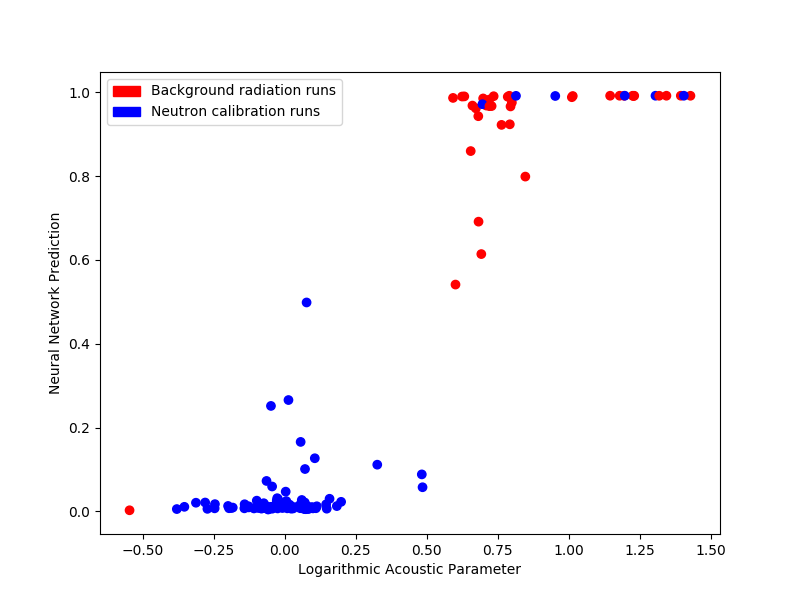
\includegraphics[width=\textwidth]{grav_opt_validation}
    \caption{\label{grav_opt_validation} Accuracy of optimal gravitational differentiation training run compared to Acoustic Parameter (98\% accuracy).}
\end{figure}

As seen in Figure \ref{grav_acc_by_hyper}, all 3 hyperparameters that were optimized during the grid search had a significant effect on accuracy:

\begin{itemize}
    \item Smaller gravitational multipliers improved performance; the best value tested was 0.0005. This implies that the gravity effect on each unlabeled event should be weighted lightly compared to the labeled examples.
    \item Higher learning rates improve performance, with the best value tested at a quite high 0.03.
    \item Larger distortion powers (which raise the confidence threshold for a significant gravitational effect) improved performance, with the best tested at 11.
\end{itemize}

\begin{figure}[h]
    \centering
    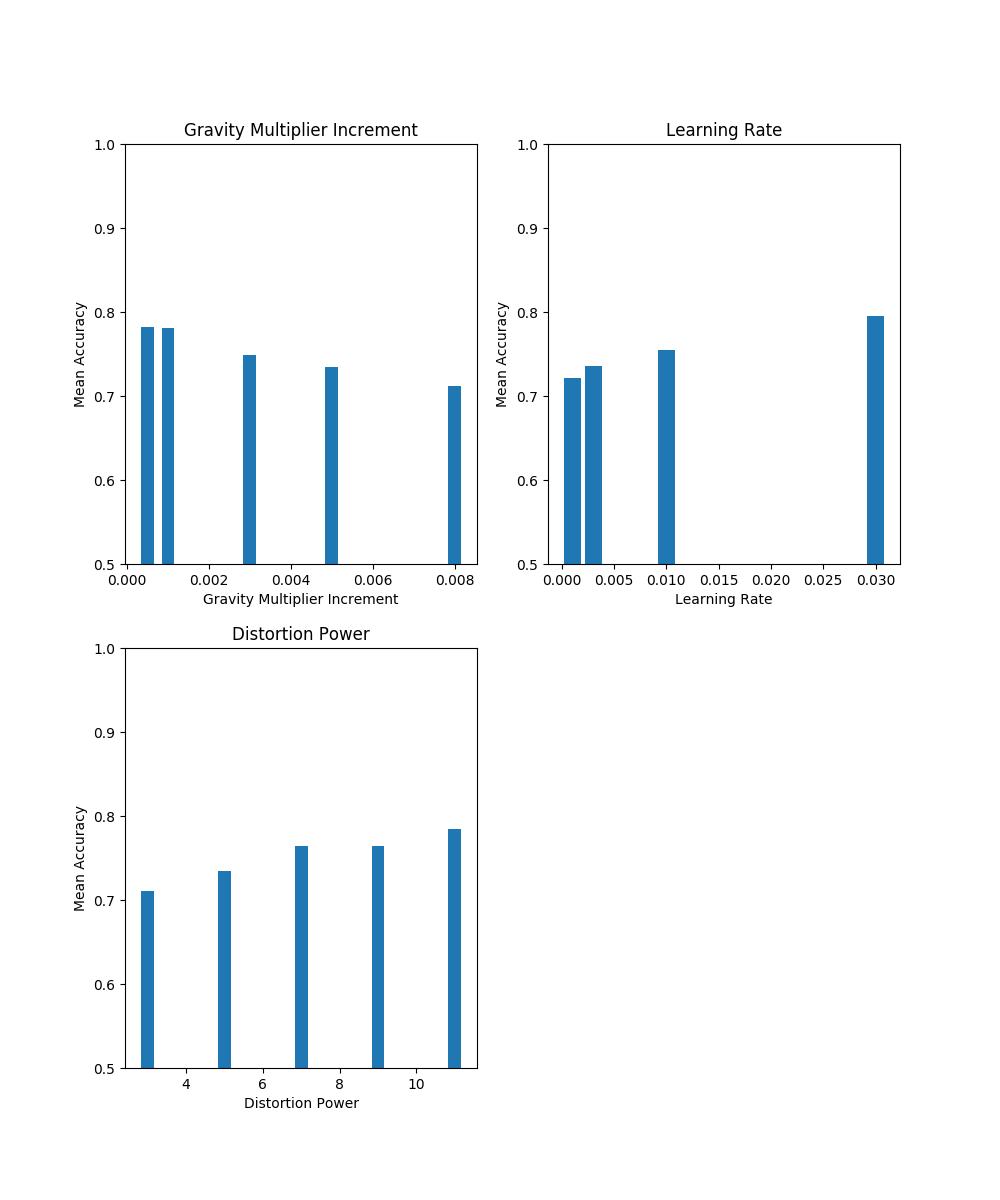
\includegraphics[width=\textwidth]{grav_acc_by_hyper}
    \caption{\label{grav_acc_by_hyper} Accuracy of gravitational differentiation as a function of hyperparameter values.}
\end{figure}

Two different options were tested with regard to size of the labeled data set $\varsigma$. Out of a set of 496 total examples available for training, either 128 (approximately $1/4$ of the total set) or 256 (approximately $1/2$) were used as labeled data. Over the entire grid search, runs with 128 examples in $\varsigma$ produced on average 64\% more errors on validation data, compared to those with 256 examples.

\subsection{Iterative Cluster Nucleation}

\subsubsection{Concept}

Iterative cluster nucleation is a semi-supervised learning algorithm that takes advantage of some amount of imperfectly labeled data, using it to classify the rest of an unlabeled training set while optimizing to produce an effective discriminator.

\subsubsection{Structure}

The algorithm is initialized as follows:

\begin{enumerate}
    \item Take a subset of the training data, referred to as the seed set $\varsigma$. Use this as the beginning of the training set.
    \item Remove classifications from any other available training examples. These create the unlabeled set $\upsilon$.
    \item Compile and randomly initialize the weights of a binary classification neural network $NN(x)$.
\end{enumerate}

Parameterized by the initial seed threshold $j$ (on the order of 0.01) and the seed threshold multiplier $k$ (on the order of 1.05), the algorithm follows these iterative steps:

\begin{enumerate}
    \item Train $NN(x)$ for 30 epochs on $\varsigma$, using the imperfect ground truth values available.
    \item Using the partially trained weights of $NN(x)$, run inference on the entirety of $\upsilon$, producing a set of predictions $p$.
    \item Find predictions within $p$ that are within a distance of $j$ of either 0 or 1; as this is a binary classifier, such a prediction represents high confidence. Remove any such examples from $\upsilon$ and add them to $\varsigma$. The principle is that, when $NN(x)$ is trained on a relatively small set for short period of time, the few predictions within $p$ that are very confident are highly likely to be correct.
    \item If no examples have been removed from $\upsilon$ and added to $\varsigma$, multiply $j$ by $k$ in place. This is done to increase the acceptance rate later in the training process, when most easily classifiable examples have been added to $\varsigma$. Otherwise, gridlock would occur, where certain examples could not be confidently classified given the training set.
\end{enumerate}

\subsubsection{Results}

During a grid search of these parameters (in addition to regularization parameters of the network), the best accuracy achieved for replication of Acoustic Parameter was exactly 100\%. The mean of all epochs within that training run was 98\%.

As seen in Figure \ref{icn_grid_search}, the network learned to replicate Acoustic Parameter very accurately. Interestingly, the examples with Acoustic Parameter values between the neutron and alpha particle ranges were also classified as such by the network. This may imply the indecisiveness on these examples is fundamental to the data rather than an implementation problem with Acoustic Parameter.

\begin{figure}[h]
    \centering
    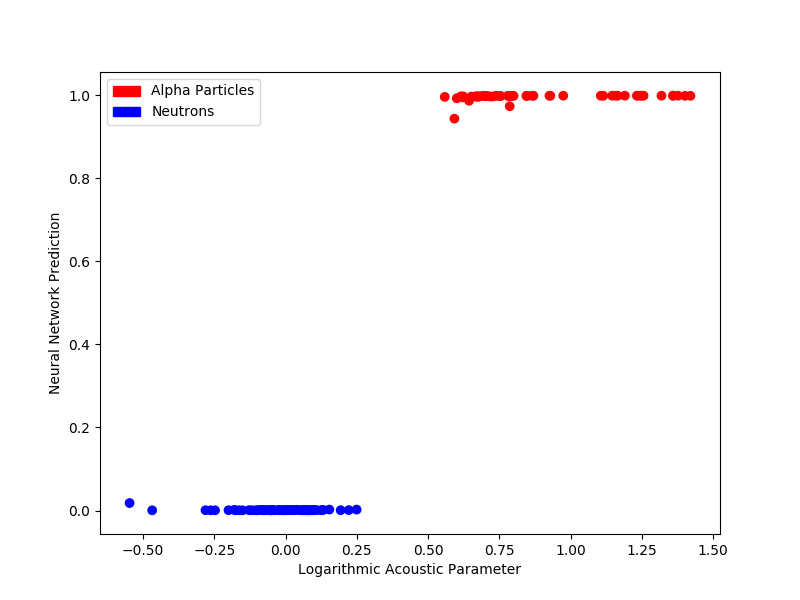
\includegraphics[width=\textwidth]{icn_grid_search}
    \caption{\label{icn_grid_search} Accuracy of optimal iterative cluster nucleation training run compared to Acoustic Parameter (100\% accuracy).}
\end{figure}

Digging deeper into the performance throughout the runs of the grid search, Figure \ref{icn_acc_by_hyper} shows the mean accuracy as a function of each of the hyperparameters that were optimized. Dropout has a clear effect, with 25\% shown to be the optimal number of neurons to drop. L2 regularization is also significant; all $\lambda$ values greater than 0 make performance worse.

\begin{figure}[h]
    \centering
    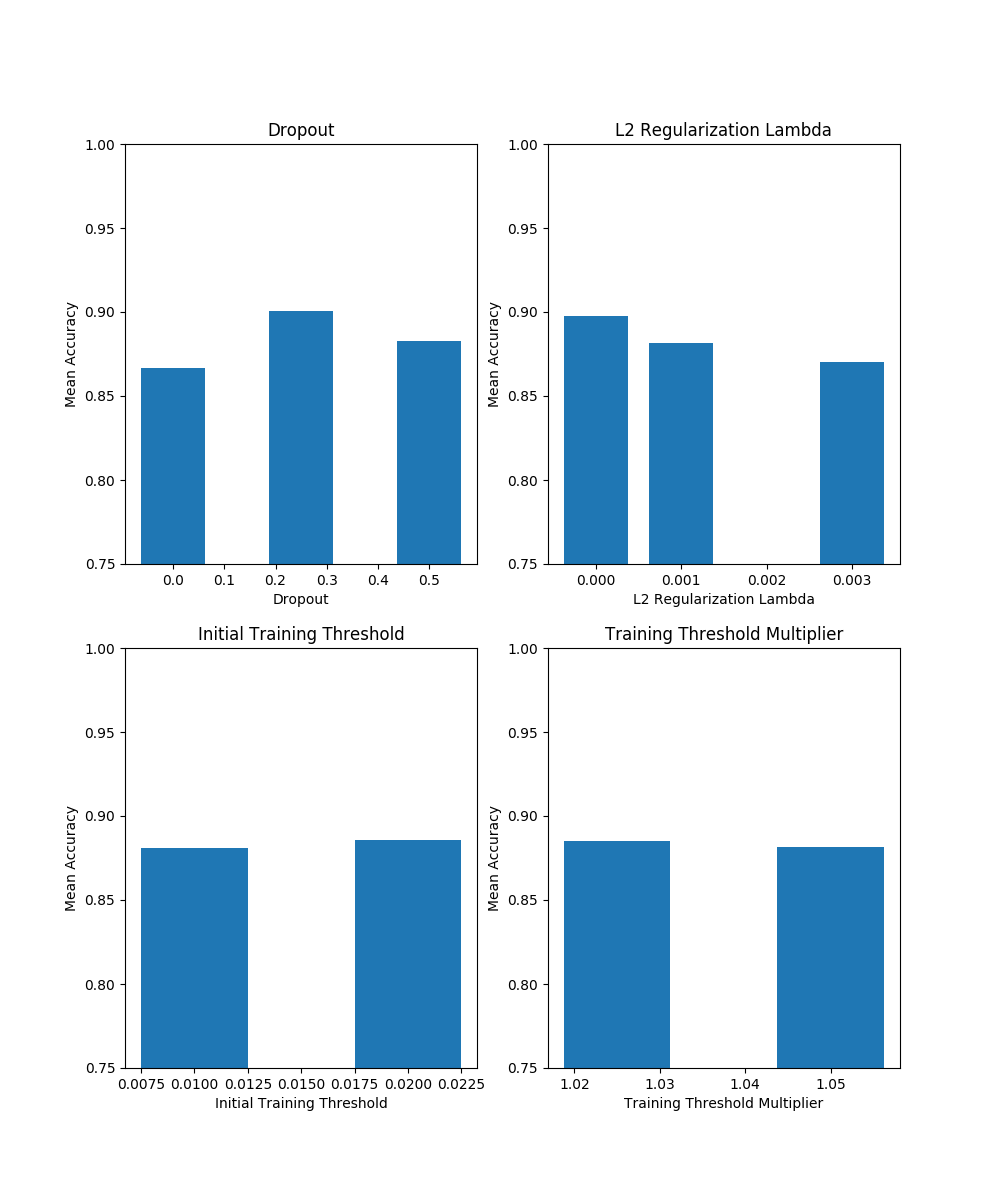
\includegraphics[width=\textwidth]{icn_acc_by_hyper}
    \caption{\label{icn_acc_by_hyper} Mean accuracy of iterative cluster nucleation as a function of hyperparameter values.}
\end{figure}

Compared to gravitational differentiation, there is a larger delta between the number of errors on the validation set depending on the number of initial training examples used. Those with 128 examples in $\varsigma$ make 85\% more errors on average. However, iterative cluster nucleation with 128 examples still makes 19\% fewer errors than gravitational differentiation with 256 examples in $\varsigma$.

\subsection{Performance Summary}

The following table directly compares performance of the semi-supervised learning systems, with the existing PICO-60 neural network provided as a baseline once again. Note that ``Max Accuracy'' refers to accuracy at replication of Acoustic Parameter, rather than replication of the ground truths.

\begin{tabular}{|l|l|l|l|}
    \hline
    Technique & Max AP Accuracy & Max Mean by Run & $\varsigma$ Errors: 128 versus 256 \\
    \hline
    Gravitational Differentiation & 98\% & 96\% & 64\% Increase \\
    \hline
    Iterative Cluster Nucleation & 100\% & 98\% & 85\% Increase \\
    \hline
\end{tabular}

\section{Conclusions}

This study has demonstrated that it is possible, using semi-supervised learning, to automatically optimize a discriminator with performance comparable to one developed and tuned by humans like Acoustic Parameter. This conclusion has been achieved through 2 rounds of optimization, the first to explore and evaluate various network structures and input formats using supervised learning, and the second to incorporate the most successful configuration into semi-supervised learning systems and replicate Acoustic Parameter as accurately as possible.

In the realm of supervised learning, it was made clear that the banded Fourier transform is the most effective input format. It produced significantly higher accuracy and tighter prediction distributions than neural networks trained on either the raw audio waveform or image window data. There is strong evidence that image data in particular does not contain sufficient information to be used for discrimination.

2 semi-supervised learning algorithms were developed, applying the best configuration found for supervised learning. While both techniques produced some very effective discriminators, iterative cluster nucleation was found to be the more effective of the 2. It replicated Acoustic Parameter with a mean of 98\% accuracy on the best configuration. This indicates that the technique shows significant promise, and may be worth consideration as a discrimination technique for future experiments.

\section{Software}

All programming for this study was done in Python 3. Keras \cite{keras}, running on a TensorFlow backend, was used for all machine learning tasks. NumPy and SciPy were used for linear algebra and signal processing. ROOT, scikit-image and scikit-learn were used for data loading and storage. Matplotlib was used for data visualization.

\printbibliography

\end{document}